\section{Evaluation}
\label{evaluation}
We evaluated our system with respect to performance and accuracy.
For the former we measure the latency of key synchronization tasks
across different network scenarios, and compare the results
with a benchmark evaluation of Dropbox. For the latter we test specific use cases
where synchronization could fail, and demonstrate that the system
properly handles these cases.

\subsection{Performance}
\label{evaluation.performance}
In order for D-Sync to be a feasible architecture
for distributed file hosting, it needs to perform comparably
to existing systems.
We therefore evaluate our prototype system with respect
to the latency of updates.
We not only show that D-Sync scales reasonably well,
but furthermore outperforms Dropbox in every evaluation.

\subsubsection{Metrics and Parameters}
In order to evaluate the latency of our system,
we measure the total time it takes for adding a single file of 
increasing size to propagate across all online clients.
We focus on adding files since these updates will necessarily
have the greatest latency, given that the system
must propagate raw file data to all online clients.
We measure the total latency as: (time stamp of when the last client receives
the entire file) - (time stamp of when the sending client starts sending the file).

We define the parameters of our performance tests in the following manner.
First, we evaluate two separate network scenarios: a LAN scenario with
two computers networked over the UO Secure wireless network,
and a WAN scenario with the same two computers on two separate home
wireless networks. 
Within these two testing scenarios,
we test additional parameters to help determine how our architecture scales.
First, we evaluate working group sizes of 2, 4, and 8 clients.
Should the system experience more than linear growth in latency
as the working group size increases, then our system will not reasonably scale.
Finally, we evaluate our system with file update sizes ranging
from $2^n$ MB, where $0 \leq n \leq 10$.
We do this in order to gain insight on how our system scales
with respect to file size.

\subsubsection{Setup}
Tests were set up in the following manner.

To evaluate D-Sync, we designate one
computer to run the broker program
and the other to run the variable number of client programs.
Though the client programs all run on the same computer,
this is a reasonable simulation of multiple computers on the same
network, as messages must travel to the broker and back. It also
eliminates the variables associated with using machines of varying
performance. In the evaluation of LAN sync, the broker is on the same
network as the clients, whereas it runs on a seperate network when
evaluation WAN sync.

To conduct a test we start the broker program, followed by the
client programs.
Once all clients are connected to the broker,
we move a text file of the appropriate
size into the workspace directory of a given client,
and measure the total time for all other clients
to receive the file.
To ensure that our measurements are correct,
we synchronize the local clocks of both computers
using the network time protocol.
We repeat the sending of text files in a serial fashion
until all files have been sent.

To evaluate Dropbox, we use the following setup.
First, we share a Dropbox folders between two users. As we only
had 2 computers with write-privelages sufficent enough to install 
Dropbox, we were only able to evaluate the 2-client scenario. Once 
our shared folder was created, we sequentially added the same test
files to one folder and used the same procedure to time the latency
between when the file was added on one client and when it finished 
writing on the other.

To prevent delta encoding advantages of Dropbox, and to simulate encoded
data, all test files consisted of randomaly generated strings of 
characters that should be statistically impossible to exist
on any of Dropbox's servers. Also, given the client-server nature of
Dropbox, we have no Dropbox LAN scenarion.
In the following section, we cover the results of these tests.

\begin{figure*}[t]
\centering
\subfigure[LAN scenario.]{
    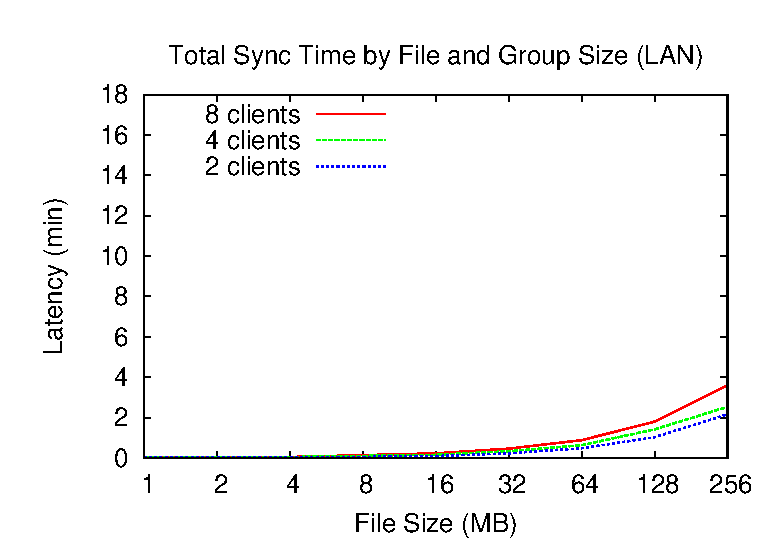
\includegraphics[scale=0.5]{figs/LAN-Online_performance.eps}
    \label{fig:LANonline}
}
~~~~\subfigure[WAN scenario.]{
    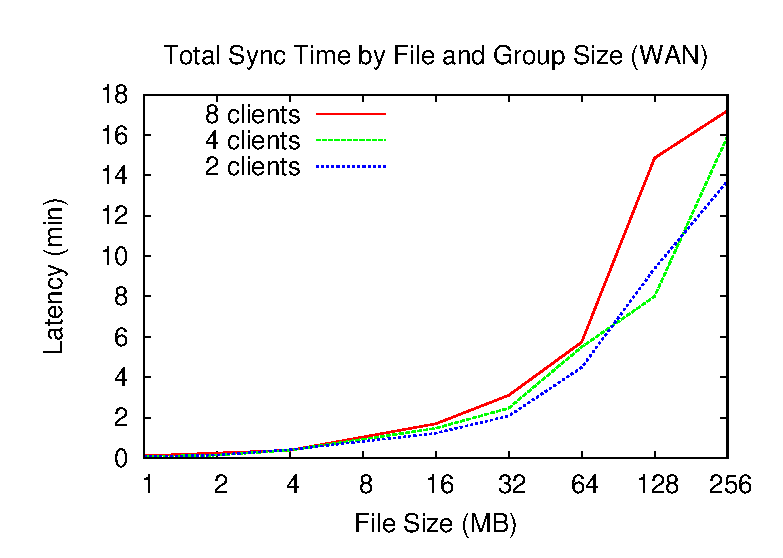
\includegraphics[scale=0.5]{figs/WAN-Online_performance.eps}
    \label{fig:WANonline}
}
\caption{\textbf{The total synchronization time for D-Sync across different network scenarios (shown in log scale).}}
\end{figure*}

\subsubsection{Scalable Synchronization}
We first analyze the total time it takes to synchronize files
across the LAN network scenario.  Figure~\ref{fig:LANonline} 
shows this synchronization latency for variable working group and
file sizes. From this graph,
we see that total synchronization time follows a linear growth pattern.
Furthermore, the latency increases only slightly with respect
to increasing working group size.
While we will need a benchmark before making a statement
on whether this is scalable,
for now we are satisfied that total synchronization time
    does not grow unreasonably.

Next we compare the results of the LAN network scenario to the WAN network scenario (\ref{fig:WANonline}.
The WAN data is considerably noisier,
reflecting variable congestion and delay in the underlying network.
However, it is still clear that total synchronization time still increases
linearly with respect to file size.
Most importantly, the data from these two networking scenarios show
that increasing numbers of clients only contributes a modest
amount of latency to our system's synchronization time.
Therefore, we find the D-Sync architecture to be scalable 
with increasing working group size.

One can clearly see that latency for file synchronization
increases significantly once we step out of a comfortable LAN
scenario to the wide area network.
But is this increase in latency reasonable with respect to existing solutions?
To determine this, we compare these results with our results
from our evaluation of Dropbox. The following graph shows that our system is
remarkable more efficient than Dropbox, which takes almost an hour and half to
sync a 256 MB file, while our system takes a modest 5 to 15 minutes to sync over
LAN and WAN, respectively. This clearly shows that the elimination of
central storage dramatically speeds up syncronization time between
any number of users.

\begin{figure}[h]
    \centering
    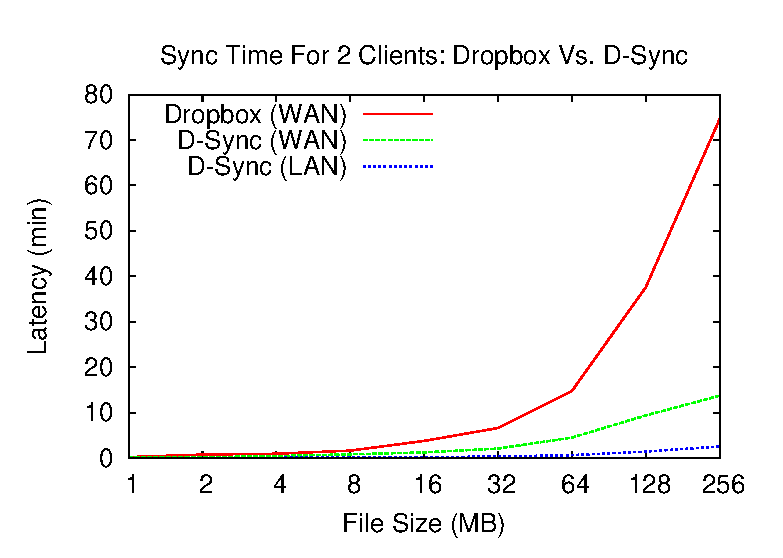
\includegraphics[scale=0.5]{figs/Dropbox_Performance.eps}
    \label{fig:dropbox}
    \caption{\textbf{A comparison of Dropbox and D-Sync's total synchronization time for two clients across network scenarios.}}
\end{figure}

\subsection{Accuracy}
\label{evaluation.accuracy}
In addition to providing an efficient solution with low latency,
it is important that our architecture provide data consistency across different
scenarios.
In other words, the system must properly synchronize
all updates across all online users.
In this section, we evaluate specific scenarios where
where the replicas in a given working group could become inconsistent across clients,
and demonstrate how our system handles these scenarios.

\subsubsection{Client Departures}
A client could depart from the system in several ways,
the most common of which are going offline and crashing.
There are three primary scenarios that could cause
data inconsistency in the event of a client departure:
\begin{enumerate}[(1)]
\item the departed client could make offline changes to his local workspace;
\item one or more online clients could make changes while the departed client is offline; or
\item both the departed client and one or more online clients could commit conflicting changes.
\end{enumerate}
In all of these cases, the system would have to properly update shared data
when the departed client returns and does an initial batch update.

We preliminarily evaluate these scenarios 
in stress tests using eight clients and one broker in a LAN setting.
We start each client and connect them to the broker,
and begin committing changes on various local workspaces.
At random intervals, we take one or more clients offline
and then bring those departed clients back after a fixed length of time (2 minutes).
Throughout the test we continue to commit changes to the local workspaces of all clients, online or offline.

Our results from four such tests show that the initial batch update
properly handles all cases of potential data inconsistency.
Across four tests, we observe 31 instances of case (1),
26 instances of case (2), and 12 instances of case (3).
In case (1), the departed client's offline changes are immediately pushed
to the broker,
who commits them to the rest of the system.
Case (2) is similarly handled;
the broker pulls up-to-date files from the nearest online client
and pushes them to the returning client.
For case (3), our prototype broker accepts the first
offline change it receives, discarding subsequent updates
with the same timestamp.
While a better solution would involve merging or handling
such conflicts in some manner,
conflict resolution strategies are beyond the scope of this work.

Furthermore, we note that our system maintains accuracy
even when other clients depart during a re-entering client's batch update.
In these cases, the second departing client
will also be updated upon return.
In this manner, all online clients will maintain a
current workspace for all online updates.
These preliminary tests show that the D-Sync architecture keeps data consistent
in the presence of arbitrary client departures.

%online race condition

%distributed broker?
